% !TEX root = /home/computer/ucsc/master-2/quarter-1/computational-fluids/master.tex
\assignment{1}{Fri 15 Oct 2021 22:42}{Assignment 1}

\subsectionfont{\fontsize{10}{10}\selectfont}

\subsection{Problem 1}%

$(F2)\Leftrightarrow(F1)\Leftrightarrow(F3)\Leftrightarrow(F4)$

By Reynolds Transport Equation
\[
(F2)\Leftrightarrow(F1)
.\] 

By divergence theorem over arbitrary volume. Can be done in either direction
\[
(F1)\Leftrightarrow(F3)
.\] 

By vector identity
\[
(F3)\Leftrightarrow(F4)
.\] 

\subsection{Problem 2}%

Consider Burgers' equation

\begin{itemize}
  \item[ \textbf{a)} ] \textbf{Multiply the equation by $2u$ and derive a new conservation law.} 
    \par Let $w(x(t),t) = u^{2}(x(t),t)$. Then
    \[
      \diff[]{w}{t} = \diff[]{u^{2}}{dt} = 2u \left( u_{x}\diff[]{x}{t} + u_{t} \right)
    .\] 

    Where $\diff[]{x}{t} = u = \sqrt{w}$ (considering only the positive root).
    So
    \begin{align*}
      \diff[]{w}{t} &= 2uu_{t} + 2u \left( \frac{u^{2}}{2} \right)_{x}
      = 0 \quad\quad (2u\cdot\text{Burgers'})\\
                    &= w_{t} + \sqrt{w}u_{x} = 0
    \end{align*}

    is the new conservation law in non-conservative form and $\sqrt{w}$ is the
    characteristic speed, and the flux function $f(w)_{x}$ satisfies
    \begin{align*}
      f(w)_{x} &= \diff[]{f}{w} \diffp[]{w}{x} =\sqrt{w}w_{x} \\
               &\implies \diff[]{f}{w} = w \\
               &\implies \boxed{f(w) = \frac{2w^{\frac{3}{2}}}{3}}
    \end{align*}

    Hence the new conservation law for $w(x(t),t) = u^{2}(x(t),t)$ is
    \[
      \boxed{w_{t}+ \left( \frac{2w^{\frac{3}{2}}}{3} \right)_{x} = 0}
    .\] 

  \item[ \textbf{b)}] \textbf{Show that the original Burgers' equation and the
    new derived equation have different weak solutions.} 
    
    \begin{proof}
      
      \par Show these two equations have different shock speeds for the Riemann
      problem $u_{l}> u_{r}$. If $u$ is a weak solution of the Riemann problem
      then across the curve of discontinuity $x=\xi(t)$, then $u$ must satisfy
      the condition
      \[
        \frac{f(u_{l}) - f(u_{r})}{u_{l}-u_{r}} = \xi'(t) = \sigma
      .\] 

      For the Burgers', we have
      \[
        \frac{ \frac{u_{l}^{2}}{2} - \frac{u_{r}^{2}}{2}}{u_{l}-u_{r}} = \sigma_1
      .\] 

      and for the new derived equation, we have
      \[
        \frac{ \frac{2u_{l}^{\frac{2}{3}}}{3}
        - \frac{2u_{r}^{\frac{2}{3}}}{3}}{u_{l}-u_{r}} = \sigma_2
      .\] 

      Since $\sigma_1 \neq \sigma_{2}$, these equations have different weak
      solutions.

    \end{proof}

\end{itemize}

\subsection{Problem 3}%

Solve Burgers' on $\R$ for small enough $t\leq t_{b}$ that allows exact
piecewise-linear weak solution with the following initial conditions:
\[
  u(x,0) = g(x) = \begin{cases}
    2 & \text{if $|x| < \frac{1}{2}$} \\
    -1 & \text{otherwise}
  \end{cases}
.\] 

%\graphicspath{{/home/computer/ucsc/master-2/quarter-1/computational-fluids/assignment_01/figures/}}
\graphicspath{{./assignment_01/figures/}}

\begin{figure}[H]
  \centering
  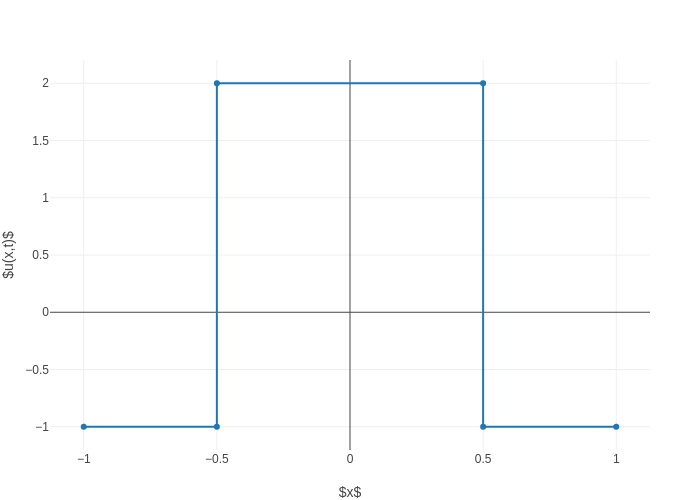
\includegraphics[width=0.8\linewidth]{init_cond.png}
  \caption{Initial Condition}%
\end{figure}

Considering parameterization $u(x(s), t(s)) \implies \diff[]{u}{s}
= \diff[]{t}{s}u_{t} + \diff[]{x}{s}u_{x}$, we get the following characteristic
equations

\[
\begin{cases}
  \diff[]{t}{s} = 1 & \implies t = s+t_0  \quad\implies t = s \\
  \diff[]{u}{s} = 0 & \implies u(s) = u_0 = u(x_0,t_0) = u(x_0,0) = g(x_0) \\
  \diff[]{x}{s} = u = g(x_0) & \implies x(s) = g(x_0)s + x_0
\end{cases}
.\] 

For $t=s$, we have $x(t) = g(x_0)t+x_0$ and $u(x,t) = g(x_0(t))$, so the
solution only depends on the initial position $x_0$. We have $2$ cases

\textbf{Case 1:} $x_0 < -\frac{1}{2}$ and $x_0 > \frac{1}{2}$,
\begin{align*}
  &\implies g(x_0) = -1 \\
  &\implies x = -t + x_0 \\
  &\implies x_0 = x + t
\end{align*}

